%%%%%%%%%%%%%%%%%%%%%%%%%%%%%%%%%%%%%%%%%%%%%%%%%%%%%%%%%%%%%%%%%%%%%%%%%%%
%% This file is part of the book
%%
%% Algorithmic Graph Theory
%% http://code.google.com/p/graphbook/
%%
%% Copyright (C) 2009--2012 Minh Van Nguyen <mvngu.name@gmail.com>
%%
%% See the file COPYING for copying conditions.
%%%%%%%%%%%%%%%%%%%%%%%%%%%%%%%%%%%%%%%%%%%%%%%%%%%%%%%%%%%%%%%%%%%%%%%%%%%

\documentclass{article}

\usepackage{pgfplots}
\usepackage{subfigure}
\usepackage{tikz}
\usetikzlibrary{external}
\tikzexternalize{Zachary-karate-club-community}

\begin{document}

\begin{figure}
\subfigure[Zachary karate club network.]{
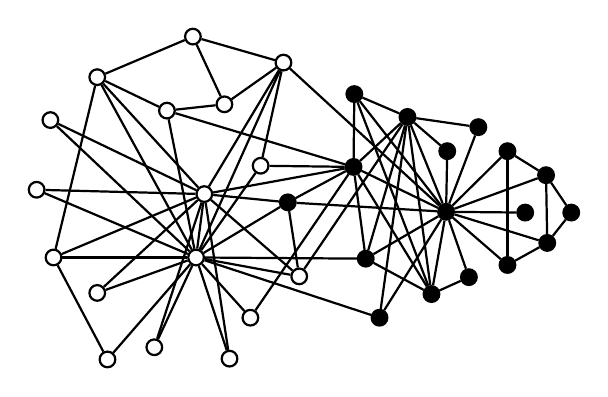
\begin{tikzpicture}
[lineDecorate/.style={-,thick},%
  nodeDecorate/.style={shape=circle,inner sep=2pt,draw,thick},
  scale=0.5]
%% community; open nodes
\foreach \nodename/\x/\y in {
  10/5.77/1.38, 15/3.33/0.63, 16/1.88/2.01, 19/0.69/6.40,
  21/0.34/4.63, 23/5.24/0.34, 24/1.88/7.49, 25/5.11/6.80,
  26/4.31/8.52, 27/2.14/0.32, 28/3.65/6.64, 29/6.03/5.24,
  30/0.77/2.91, 31/7.01/2.43, 32/6.61/7.86, 33/4.60/4.52,
  34/4.39/2.91}
{
  \node (\nodename) at (\x,\y) [nodeDecorate] {};
}
%% community; filled nodes
\foreach \nodename/\x/\y in {
  1/10.74/4.07, 2/9.76/6.48, 3/8.39/5.21, 4/10.37/1.98, 5/12.30/5.61,
  6/13.31/3.28, 7/13.28/5.00, 8/8.41/7.06, 9/6.72/4.31, 11/12.30/2.72,
  12/12.75/4.05, 13/11.32/2.41, 14/8.70/2.88, 17/13.92/4.05,
  18/10.77/5.61, 20/9.05/1.38, 22/11.56/6.22}
{
  \node (\nodename) at (\x,\y) [nodeDecorate,fill=black] {};
}
%% edges or lines
\path
\foreach \startnode/\endnode in {
  1/2, 1/3, 1/4, 1/5, 1/6, 1/7, 1/8, 1/9, 1/11, 1/12, 1/13, 1/14,
  1/18, 1/20, 1/22, 1/32, 2/3, 2/4, 2/8, 2/14, 2/18, 2/20, 2/22, 2/31,
  3/4, 3/8, 3/9, 3/10, 3/14, 3/28, 3/29, 3/33, 4/8, 4/13, 4/14, 5/7,
  5/11, 6/11, 6/17, 6/7, 7/17, 9/31, 9/33, 9/34, 10/34, 14/34, 15/33,
  15/34, 16/33, 16/34, 19/33, 19/34, 20/34, 21/33, 21/34, 23/33,
  23/34, 24/26, 24/28, 24/30, 24/33, 24/34, 25/26, 25/28, 25/32,
  26/32, 27/30, 27/34, 28/34, 29/32, 29/34, 30/33, 30/34, 31/33,
  31/34, 32/33, 32/34, 33/34}
{
  (\startnode) edge[lineDecorate] node {} (\endnode)
};
\end{tikzpicture}
}
\end{figure}

\end{document}
